
%(BEGIN_QUESTION)
% Copyright 2011, Tony R. Kuphaldt, released under the Creative Commons Attribution License (v 1.0)
% This means you may do almost anything with this work of mine, so long as you give me proper credit

Many flammable gases are produced in chemical processing and oil refineries as ``waste'' products.  These ``waste'' gases may be used as fuel for steam boilers and combustion heaters in other parts of the refinery.  The problem is, ``waste'' fuel gas production is often unsteady, and the demand for fuel gas in boilers and heaters is unsteady as well.  There are times when there will be a surplus of waste gas (more than can be used), and times when there will not be enough.

The following pressure control system works to maintain constant fuel gas pressure in the accumulator vessel despite changes in waste gas flows and fuel gas demands:

$$\includegraphics[width=15.5cm]{i01526x01.eps}$$

Identify the proper split-ranges for control valves PV-45a and PV-45b, given the purpose of the control system and the necessary fail-safe modes for each valve as shown in the P\&ID, assuming they are driven off the exact same 4-20 mA signal from PIC-45.  Also, determine the necessary action (direct or reverse) for PIC-45:

% No blank lines allowed between lines of an \halign structure!
% I use comments (%) instead, so that TeX doesn't choke.

$$\vbox{\offinterlineskip
\halign{\strut
\vrule \quad\hfil # \ \hfil & 
\vrule \quad\hfil # \ \hfil & 
\vrule \quad\hfil # \ \hfil \vrule \cr
\noalign{\hrule}
%
% First row
{\bf Valve} & {\bf Fully closed at} & {\bf Fully open at} \cr
 & (mA) & (mA) \cr
%
\noalign{\hrule}
%
% Another row
PV-45a &  &  \cr
%
\noalign{\hrule}
%
% Another row
PV-45b &  &  \cr
%
\noalign{\hrule}
} % End of \halign 
}$$ % End of \vbox

Suppose an operator shut the flare line block valve during the last ``turnaround'' (complete system shut-down for maintenance), locking it in place and labeling the valve with a safety tag (lock-out, tag-out), then forgetting to unlock and open the valve prior to system start-up.  What effect would this locked valve have on the operation of the system?  What process symptoms, if any, would indicate that the flare block valve was still shut?  What would be the proper way to remove the operator's lock and tag so that the block valve could be opened?

\vskip 20pt \vbox{\hrule \hbox{\strut \vrule{} {\bf Suggestions for Socratic discussion} \vrule} \hrule}

\begin{itemize}
\item{} Explain the possible rationale for closing and locking the flare block valve during the turnaround.
\item{} Describe how this pressure control system will respond if PT-45 fails with a high signal.
\item{} Describe how this pressure control system will respond if the instrument air to FV-45a fails.
\item{} Describe how this pressure control system will respond if the instrument air to FV-45b fails.
\end{itemize}

\underbar{file i01526}
%(END_QUESTION)





%(BEGIN_ANSWER)

\noindent
{\bf Partial answer:}

% No blank lines allowed between lines of an \halign structure!
% I use comments (%) instead, so that TeX doesn't choke.

$$\vbox{\offinterlineskip
\halign{\strut
\vrule \quad\hfil # \ \hfil & 
\vrule \quad\hfil # \ \hfil & 
\vrule \quad\hfil # \ \hfil \vrule \cr
\noalign{\hrule}
%
% First row
{\bf Valve} & {\bf Fully closed at} & {\bf Fully open at} \cr
 & (mA) & (mA) \cr
%
\noalign{\hrule}
%
% Another row
PV-45a & 12 mA &  \cr
%
\noalign{\hrule}
%
% Another row
PV-45b & 12 mA &  \cr
%
\noalign{\hrule}
} % End of \halign 
}$$ % End of \vbox

A strong indication of the block valve being left shut is accumulator pressure significantly greater than setpoint with FV-45b wide open.

%(END_ANSWER)





%(BEGIN_NOTES)

% No blank lines allowed between lines of an \halign structure!
% I use comments (%) instead, so that TeX doesn't choke.

$$\vbox{\offinterlineskip
\halign{\strut
\vrule \quad\hfil # \ \hfil & 
\vrule \quad\hfil # \ \hfil & 
\vrule \quad\hfil # \ \hfil \vrule \cr
\noalign{\hrule}
%
% First row
{\bf Valve} & {\bf Fully closed at} & {\bf Fully open at} \cr
 & (mA) & (mA) \cr
%
\noalign{\hrule}
%
% Another row
PV-45a & 12 mA & 20 mA \cr
%
\noalign{\hrule}
%
% Another row
PV-45b & 12 mA & 4 mA \cr
%
\noalign{\hrule}
} % End of \halign 
}$$ % End of \vbox

$$\includegraphics[width=15.5cm]{i01526x02.eps}$$

It should be noted that the shut flare block valve would not manifest any symptoms unless the pressure control system had need to vent to the flare (i.e. the waste gas supply exceeded the fuel gas demand).














\vskip 20pt \vbox{\hrule \hbox{\strut \vrule{} {\bf Virtual Troubleshooting} \vrule} \hrule}

This question is a good candidate for a ``Virtual Troubleshooting'' exercise.  Presenting the diagram to students, you first imagine in your own mind a particular fault in the system.  Then, you present one or more symptoms of that fault (something noticeable by an operator or other user of the system).  Students then propose various diagnostic tests to perform on this system to identify the nature and location of the fault, as though they were technicians trying to troubleshoot the problem.  Your job is to tell them what the result(s) would be for each of the proposed diagnostic tests, documenting those results where all the students can see.

During and after the exercise, it is good to ask students follow-up questions such as:

\begin{itemize}
\item{} What does the result of the last diagnostic test tell you about the fault?
\item{} Suppose the results of the last diagnostic test were different.  What then would that result tell you about the fault?
\item{} Is the last diagnostic test the best one we could do?
\item{} What would be the ideal order of tests, to diagnose the problem in as few steps as possible?
\end{itemize}


%INDEX% Basics, control loop troubleshooting: determining cause of control problem
%INDEX% Final Control Elements, valve: split-ranging

%(END_NOTES)


